\documentclass[12pt,a4paper]{article}
\usepackage[UTF8]{ctex}
\usepackage[T1]{fontenc}
\usepackage{graphicx}
\usepackage{authblk}
\usepackage{hyperref}
\usepackage{fontspec}
\usepackage{fancyhdr}

\hypersetup{
    hidelinks,
	colorlinks=true,
	allcolors=black,
	pdfstartview=Fit,
	breaklinks=true
}

\usepackage{listings} % 插入代码用到

% 用来设置附录中代码的样式
\lstset{
	basicstyle          =   \sffamily,          % 基本代码风格
	keywordstyle        =   \bfseries,          % 关键字风格
	commentstyle        =   \rmfamily\itshape,  % 注释的风格,斜体
	stringstyle         =   \ttfamily,  % 字符串风格
	flexiblecolumns,                % 别问为什么,加上这个
	numbers             =   left,   % 行号的位置在左边
	showspaces          =   false,  % 是否显示空格,显示了有点乱,所以不现实了
	numberstyle         =   \zihao{-5}\ttfamily,    % 行号的样式,小五号,tt等宽字体
	showstringspaces    =   false,
	captionpos          =   t,      % 这段代码的名字所呈现的位置,t指的是top上面
	frame               =   lrtb,   % 显示边框
}

\lstdefinestyle{Python}{
	language        =   Python, % 语言选Python
	basicstyle      =   \zihao{-5}\ttfamily,
	numberstyle     =   \zihao{-5}\ttfamily,
	keywordstyle    =   \color{blue},
	keywordstyle    =   [2] \color{teal},
	stringstyle     =   \color{magenta},
	commentstyle    =   \color{red}\ttfamily,
	breaklines      =   true,   % 自动换行,建议不要写太长的行
	columns         =   fixed,  % 如果不加这一句,字间距就不固定,很丑,必须加
	basewidth       =   0.5em,
}


\title{P大树洞生成器设计与实现}
\author[1]{匡宇轩(2100013089)}
\author[1]{陈红韵(2100013130)}
\author[2]{王天源(1700017703)}
\affil[1]{北京大学信息科学技术学院}
\affil[2]{北京大学元培学院}
\date{2022年6月}

\begin{document}

\pagestyle{fancy}
\fancyhead[L]{}
\fancyhead[R]{}
\fancyhead[C]{\small 北京大学《AI引论》课程小组项目书面报告(2021-2022,春季学期)}

\maketitle
\newpage
\renewcommand{\abstractname}{\large 摘要}
\begin{abstract}
\normalsize
    本项目为北京大学信息科学技术学院国家精品课程《人工智能引论》的课程项目。本文为该项目的总结报告。
    
    本项目受到北京大学树洞的启发。树洞作为匿名交流论坛,是一个天然的自然语言处理语料库(在遵守相关规定的情况下)。

    本项目基于因果语言建模(CLM)的原理开发,使用Python和PyTorch实现。

    我们在树洞文本数据集上训练LSTM模型,并根据用户的输入,使用训练好的模型产生回复。我们将模型命名为 HoleAI。

\end{abstract}

\textbf{关键词:自然语言处理;长短期记忆网络;因果语言建模}

\newpage
\tableofcontents


\section{背景介绍}
P大树洞作为校内学生匿名交流平台,是一个完美的语料库(在遵守相关规定的情况下),十分适合NLP相关任务。

本项目通过收集大量树洞文本数据,用神经网络进行拟合,希望能创造出一个具有P大学生气质的AI。

使用者可以作为“洞主”,模拟发树洞的过程,但是回复的字母君都是AI自动生成。
\section{相关工作}
\subsection{\href{https://arxiv.org/abs/1301.3781}{Word2Vec}}
该工作提出了两种新颖的模型架构,用于从非常大的数据集中计算单词的连续向量表示。这些表示的质量是在单词相似度任务中测量的,并将结果与以前基于不同类型神经网络的最佳性能技术进行比较。

研究者观察到本方法以更低的计算成本显着提高了准确性,即从 16 亿个单词数据集中学习高质量的单词向量只需不到一天的时间。此外,该工作表明这些向量在测试集上提供了最先进的性能,用于测量句法和语义词的相似性。\cite{ref1}
% (1). \href{https://arxiv.org/abs/1301.3781}{Word2Vec} 提供了2种将词转化为稠密向量表示的方法,便于神经网络的输入。
\subsection{\href{https://pubmed.ncbi.nlm.nih.gov/9377276/}{LSTM}}
通过循环反向传播学习在较长的时间间隔内存储信息需要很长时间,主要是因为不足的、衰减的梯度回传。

该工作简要回顾了 Hochreiter (1991) 对这个问题的分析,然后通过引入一种新的、有效的、基于梯度的方法来解决这个问题,称为长短期记忆 (LSTM)。

通过在不造成伤害的情况下截断梯度,LSTM 可以通过在特殊单元内通过恒定误差轮播强制恒定误差流来学习弥合超过 1000 个离散时间步长的最小时间滞后。

与实时循环学习、随时间的反向传播、循环级联相关、Elman 网络和神经序列分块相比,LSTM 运行更加成功,并且学习速度更快。LSTM 还解决了以前的循环网络算法从未解决过的复杂、人为的长时间滞后任务。\cite{ref2}
% (2). \href{https://pubmed.ncbi.nlm.nih.gov/9377276/}{LSTM},又称“长短期记忆网络”,是一种可以学习长期序列的循环神经网络,广泛应用于语言模型中。


\section{项目细节}
本项目的基本框架为:

(1). 数据集收集与预处理

(2). 神经网络构建与训练

(3). 前端可视化、人机交互

\subsection{数据集收集与预处理}
    鉴于P大树洞的相关管理规范,很遗憾我们无法使用爬虫技术获取数据集,因此我们采用了手动收集的方式收集数据。
    
    经过收集,我们获取了一份包含3000余条树洞,约一百万字的树洞文本,其中包含了三部分:日常话题、经典话题和神洞(即回复量较多的树洞)。
    
数据收集完毕后,我们对数据进行了清洗。主要包括:去除洞号、回复数、收藏数等无用信息;去除出现频率过低的字符;去除大量重复的字符。
    
    数据集格式如图1所示。
    
    \begin{figure}[!h]
        \centering
    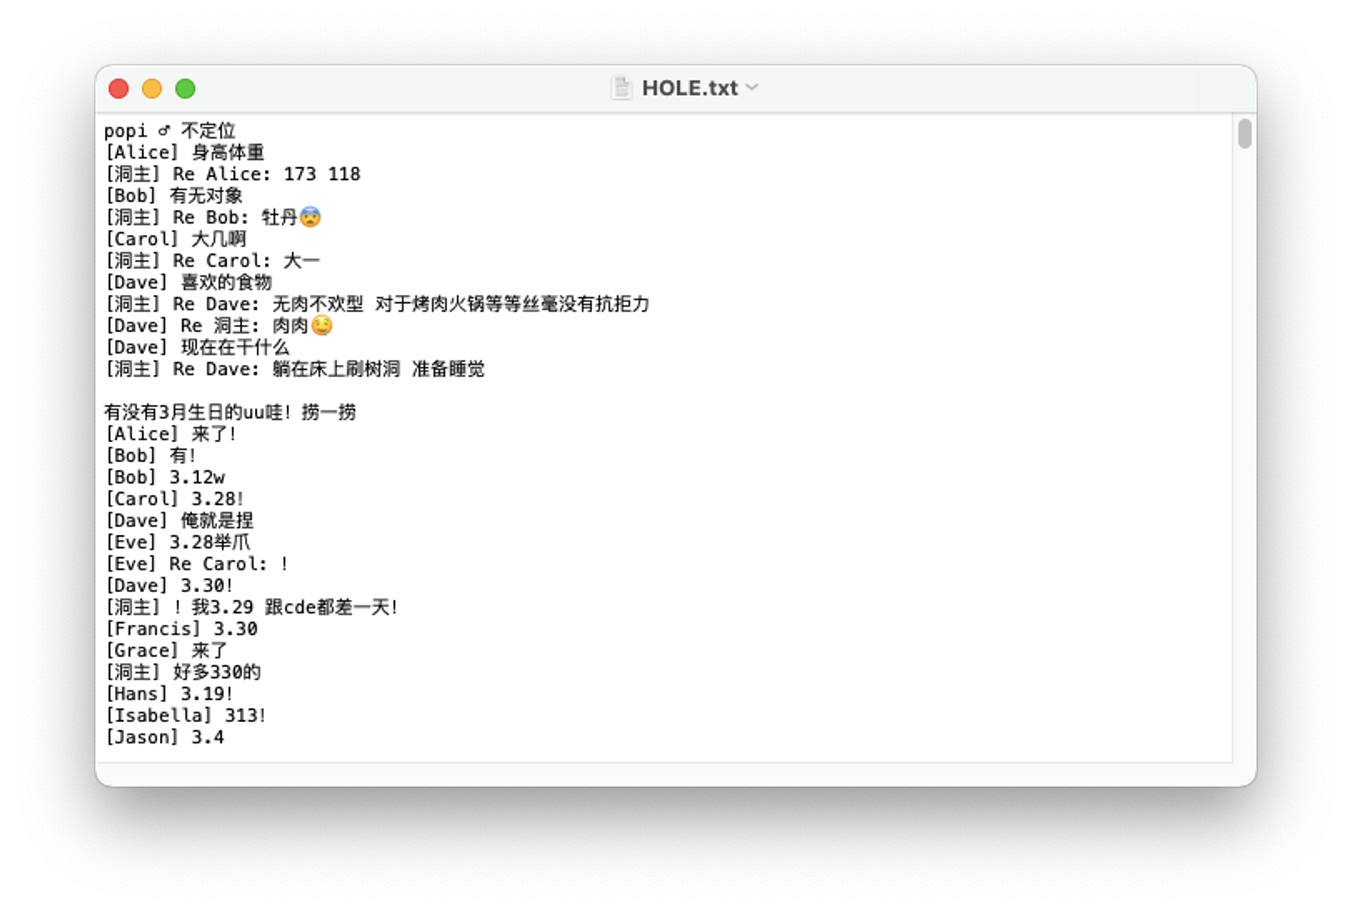
\includegraphics[width=0.5\textwidth]{图片6.png}
        \caption{数据集}
    \end{figure}
    
    接着我们利用 \verb|gensim.models.Word2Vec|构建字符到索引的双射,从而将每个字符都表示为一个One-hot vector,作为训练的初始输入。
\subsection{LSTM介绍}
    LSTM,中文为“长短期记忆网络”,是一种循环神经网络,可以学习和预测时间序列。
    
相较于普通的RNN (如图2),LSTM的优势在于其可以保持长时间的记忆,并且可以根据监督灵活的选择是否“忘记”,从而可以持久的保存语义信息。这在文本生成的工作中十分重要。
    
    \begin{figure}[!h]
        \centering
        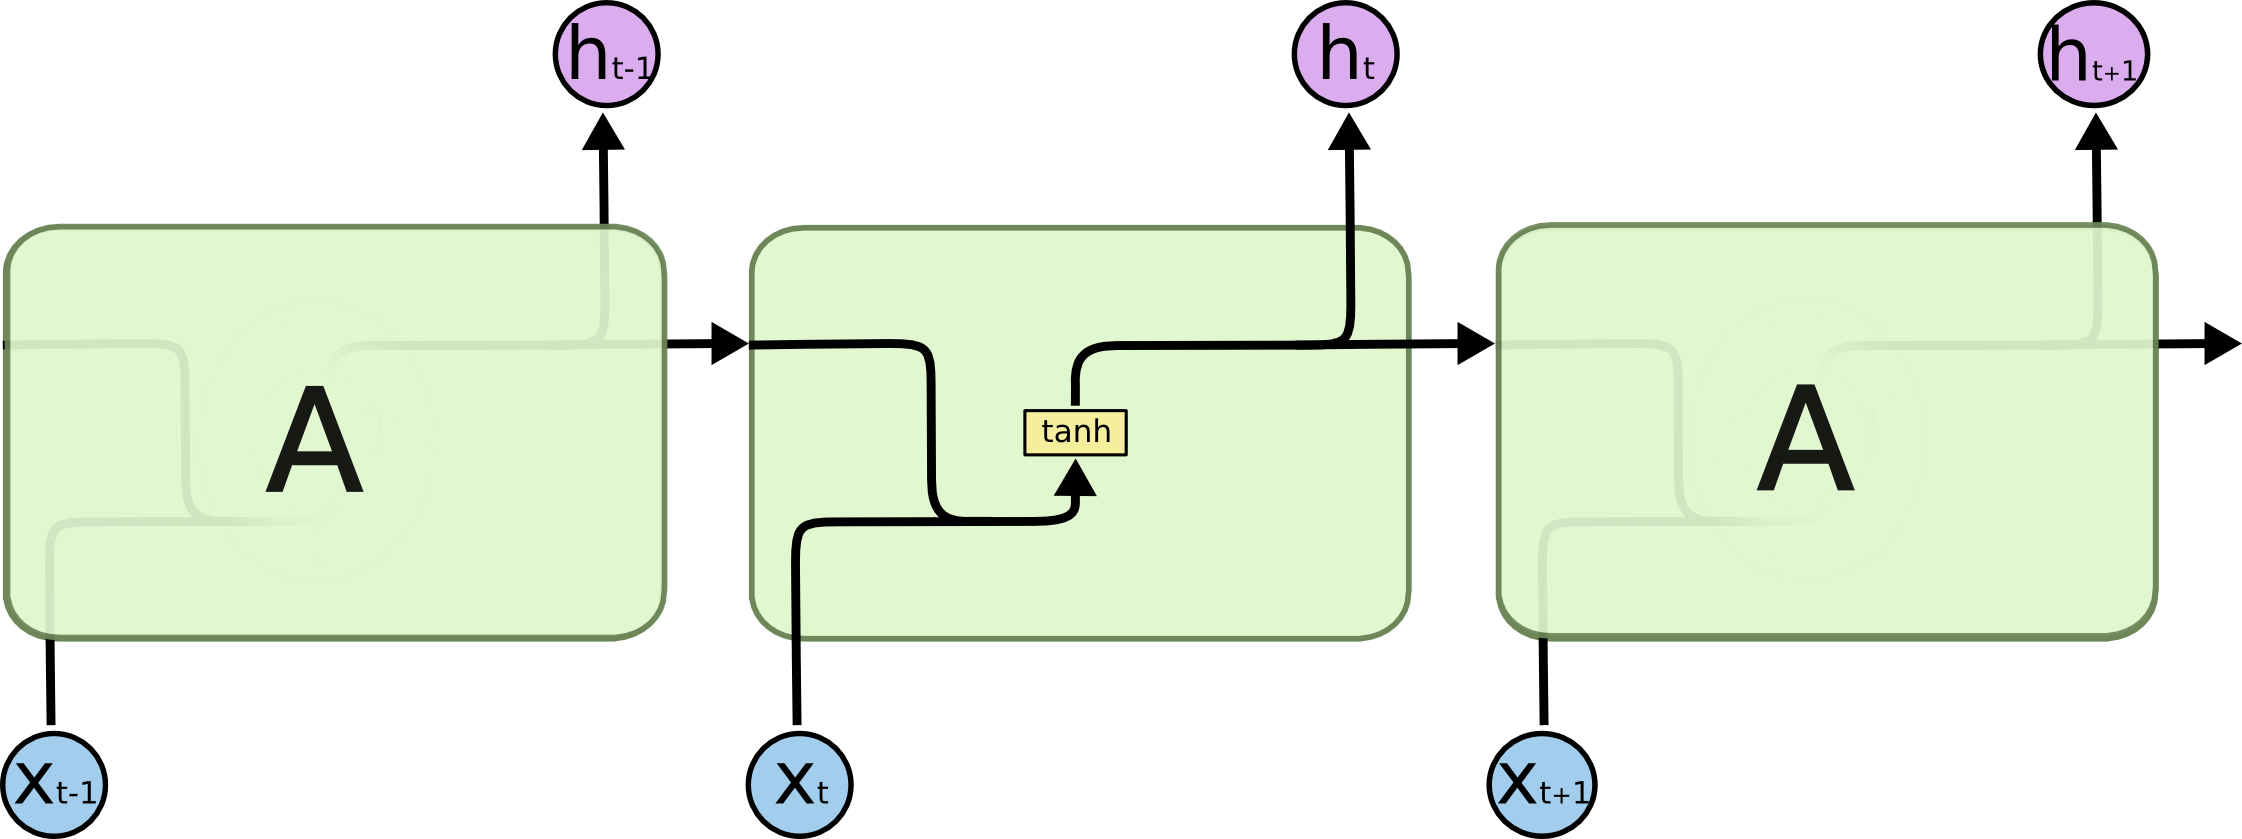
\includegraphics[width=0.5\textwidth]{图片8.png}
        \caption{Vanilla RNN}
    \end{figure}
    
    LSTM除了可以学习长序列外,还能够进行一次多步预测,对于时间序列预测有一定参考价值。
    
    LSTM记忆长期记忆的秘密在于门控,每个LSTM单元内有三道门,分别为输入门、遗忘门和输出门。

    输入门:
    
    $f_{t}=\sigma\left(W_{f} \cdot\left[h_{t-1}, x_{t}\right]+b_{f}\right)$
    
    遗忘门:
    
    $i_{t}=\sigma\left(W_{i} \cdot\left[h_{t-1}, x_{t}\right]+b_{i}\right)$
    
    $\tilde{C}_{t}=\tanh \left(W_{C} \cdot\left[h_{t-1}, x_{t}\right]+b_{C}\right)$
    
    $C_{t}=f_{t} * C_{t-1}+i_{t} * \tilde{C}_{t}$
    
    输出门:
    
    $o_{t}=\sigma\left(W_{o}\left[h_{t-1}, x_{t}\right]+b_{o}\right)$
    
    $h_{t}=o_{t} * \tanh \left(C_{t}\right)$
    
   其基本单元如图3所示。\cite{ref3}
    \begin{figure}[!h]
        \centering
        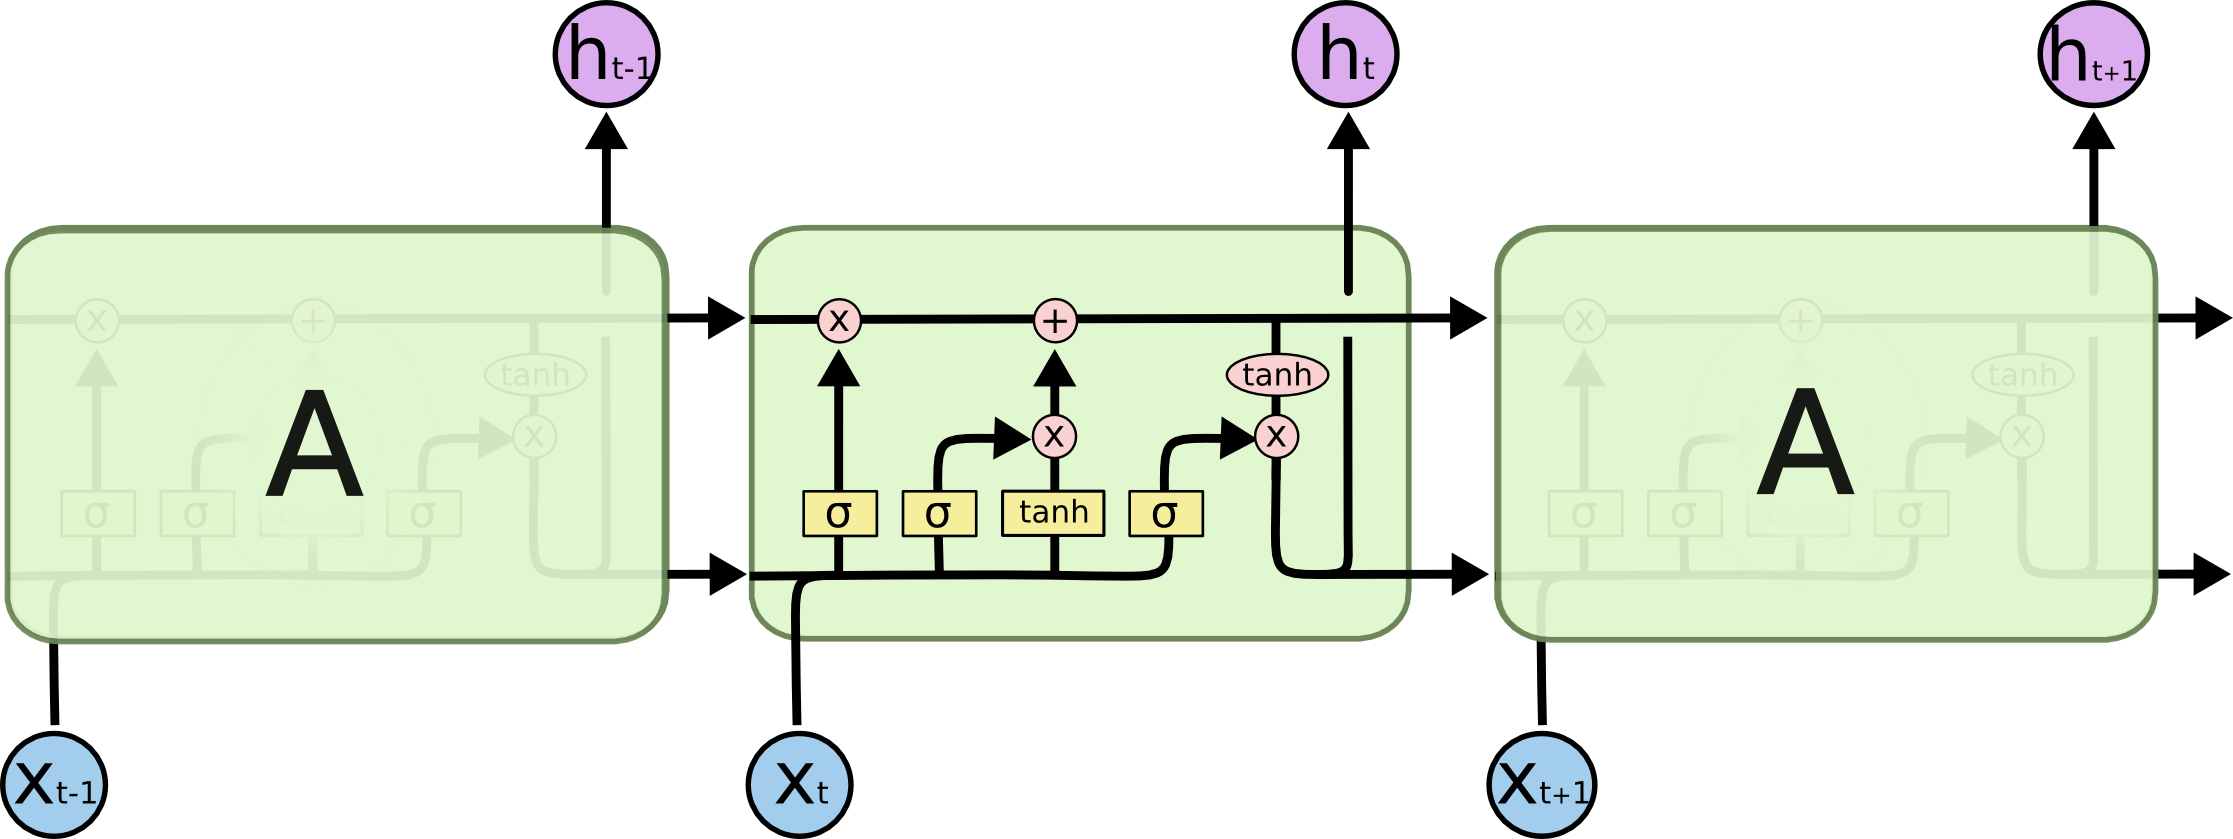
\includegraphics[width=0.5\textwidth]{图片7.png}
        \caption{LSTM单元}
    \end{figure}

    更进一步,我们将LSTM的隐藏层输出再次输入新的LSTM单元,便类似全连接层构造出了多层LSTM (Stacked LSTM),如图4所示。

    \begin{figure}[!h]
        \centering
        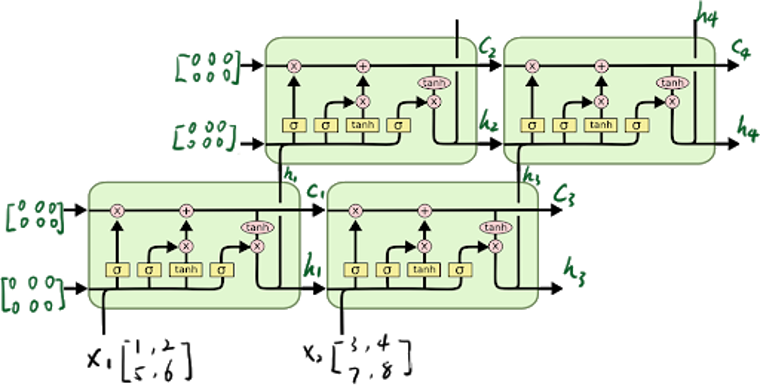
\includegraphics[width=0.5\textwidth]{图片1.png}
        \caption{Stacked LSTM}
    \end{figure}


\subsection{神经网络构建}
    我们的输入是批量化的由截断的原始文本映射而来的One-hot vectors,其稀疏性不利于训练,所以我们首先将其通过Embedding层,转为dense vectors。
    
    接着我们依次将其通过Stacked LSTM,Layer Normalization,Fully-Connected Layer,形成与原向量维度一致的输出向量。
    
    接着我们将其通过Softmax层形成概率分布,将其与原始的One-hot vectors进行交叉熵损失函数计算,再利用梯度进行Backpropagation through time进行参数更新。
    
    完整的Pipeline如图5所示。
\begin{figure}[!h]
    \centering
    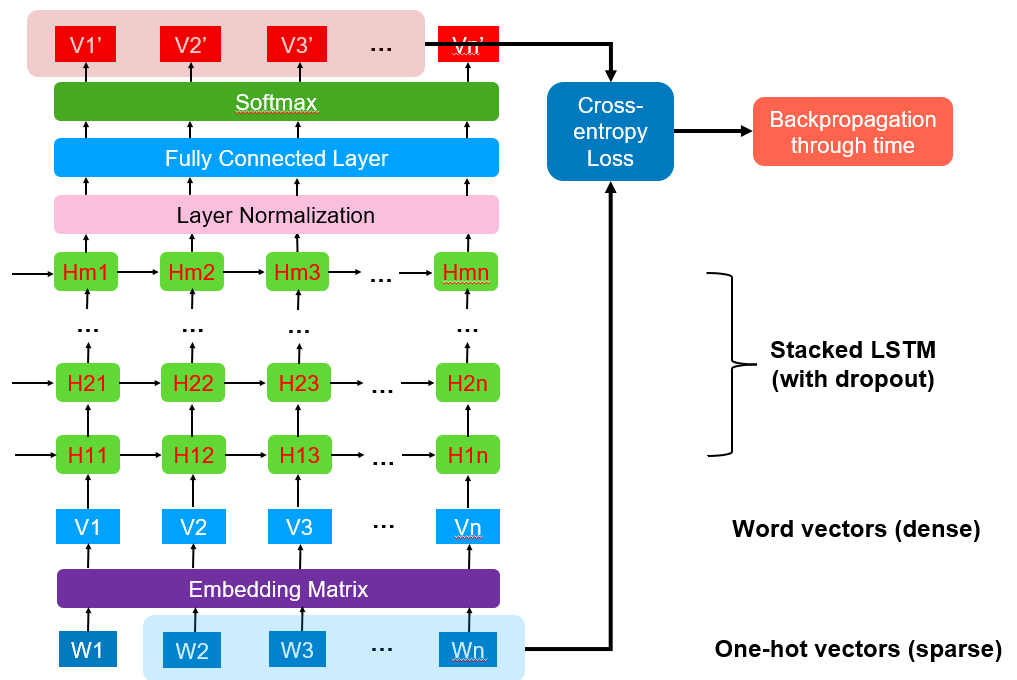
\includegraphics[width=1\textwidth]{图片3.png}
    \caption{Whole Pipeline}
\end{figure}

\subsection{神经网络训练}
    我们使用树洞文本语料库对模型从头开始训练。
    
    算力平台为北大人工智能集群系统,使用RTX 3080进行训练。训练时间大致为4 hours per 50 epochs,这也与模型的超参数有关。
    
    训练记录截图如图6所示。
    
    \begin{figure}[!h]
        \centering
        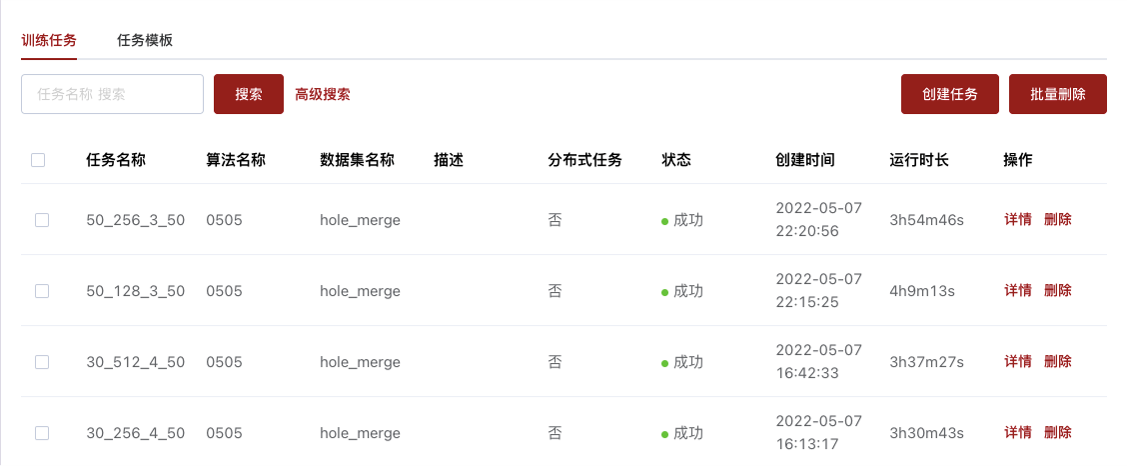
\includegraphics[width=1\textwidth]{图片4.png}
        \caption{训练记录}
    \end{figure}


\section{实验结果与分析}
\subsection{实验结果}
我们使用 \verb|tensorboard|绘制了训练过程中 \verb|train loss|, \verb|validation loss|与 \verb|epoch|的曲线图,曲线图总览如图7所示。

\begin{figure}[!h]
        \centering
        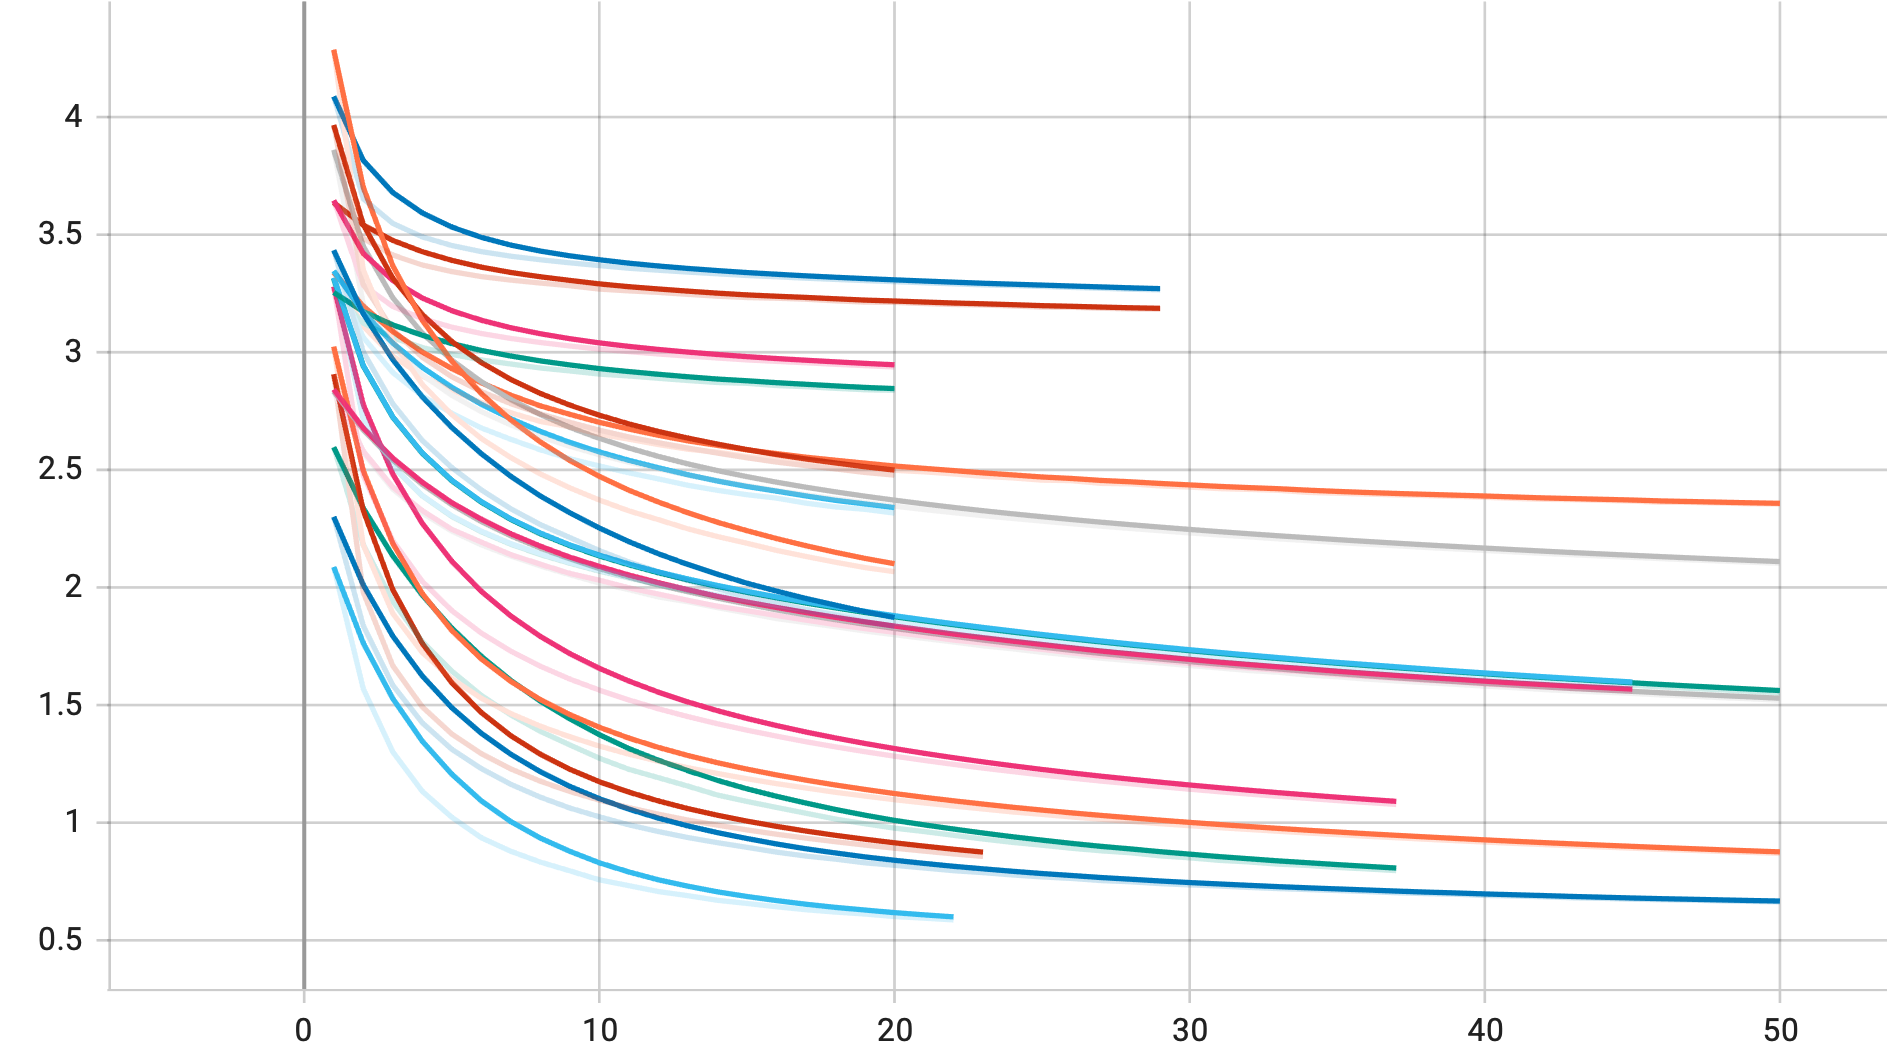
\includegraphics[width=1\textwidth]{图片9.png}
        \caption{训练结果总览}
\end{figure}

更多实验结果,如训练日志等,详见附录。

\subsection{结果分析}
我们取出其中较有代表性的三对曲线进行分析,如图8所示。

\begin{figure}[!h]
        \centering
        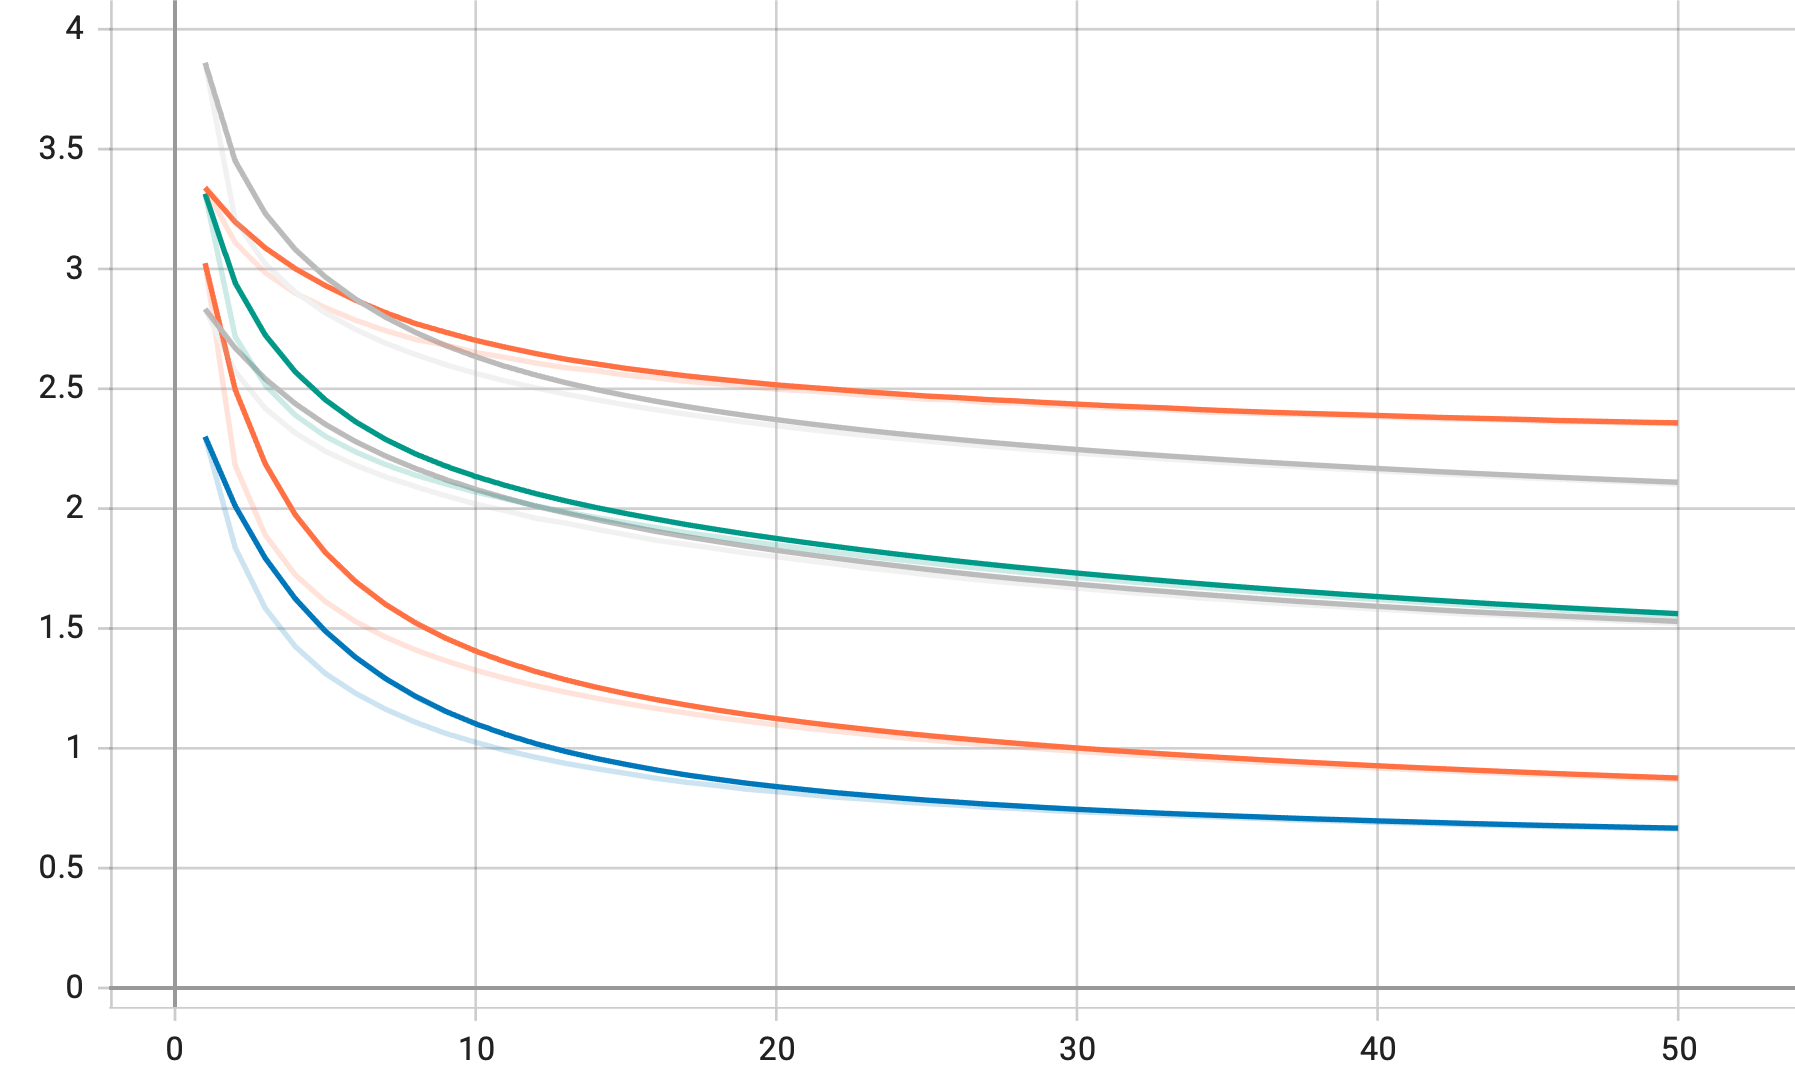
\includegraphics[width=1\textwidth]{图片10.png}
        \caption{分析曲线}
\end{figure}

我们从曲线中可以得出如下结论:

(1). 训练效果较好,损失函数值单调下降,且收敛到了一个比较低的水平。

(2). 随机分割数据集可以起到一定正则化的作用,这使得训练最后 \verb|validation loss|低于 \verb|train loss|。

我们在反复训练和调参中也总结出如下结论:

(1). Dropout rate不宜过大,LSTM堆叠层数不宜过多。否则会出现梯度消失现象,不利于参数更新。

(2). 随机split数据集,可以起到一定正则化的作用,但也因此丢失了部分语义信息。

(3). 隐层大小至关重要。隐空间越大,模型的表现力越强,对数据的拟合能力越强。

\subsection{模型生成}

我们使用训练好的模型对输入产生响应,生成回复。生成样例如图9、图10所示。

\begin{figure}[!h]
        \centering
        
\includegraphics[width=0.5\textwidth]{回复1.png}
        \caption{生成样例1}
\end{figure}

\begin{figure}[!h]
        \centering
        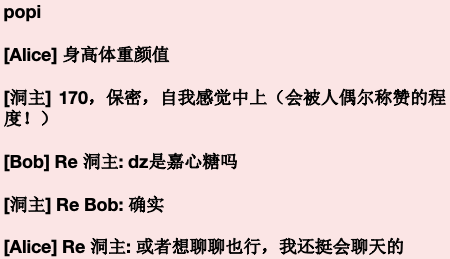
\includegraphics[width=0.5\textwidth]{回复2.png}
        \caption{生成样例2}
\end{figure}

可以看出,模型产生的回复捕捉到了文本格式,例如 \verb|[Alice]|, \verb|[Bob]|等人名格式与 \verb|Re 洞主: |等回复格式。此外,模型生成的回复在语言风格上也与真实的树洞文本有很高的相似性。即,“有内味了”。

然而,模型的生成依旧存在一定问题。如:

(1). 自说自话:即前后回复语义相关性较弱,或完全无关。

(2). 指鹿为马:即模型的回复指向性有误。

(3). 虚空索敌:即模型会对未出现的事物进行评论。

(4). 过拟合现象依旧存在:在较长文本的生成中,模型往往会“照抄”原文,产生大段已有文字。这说明模型的泛化能力依然有待提升。

\subsection{模型部署与可视化}
模型训练完成后,我们希望能用更加方便与美观的形式呈现模型的实际效果,也希望以此模拟树洞,故我们依托 \verb|GitHub Pages|和 \verb|streamlit|框架开发了本项目的前端界面。

用户点击 \href{https://kryptonite.work/pkuhole/}{https://kryptonite.work/pkuhole/} 链接即可进入本项目的网站,界面如图11所示。

\begin{figure}[!h]
        \centering
        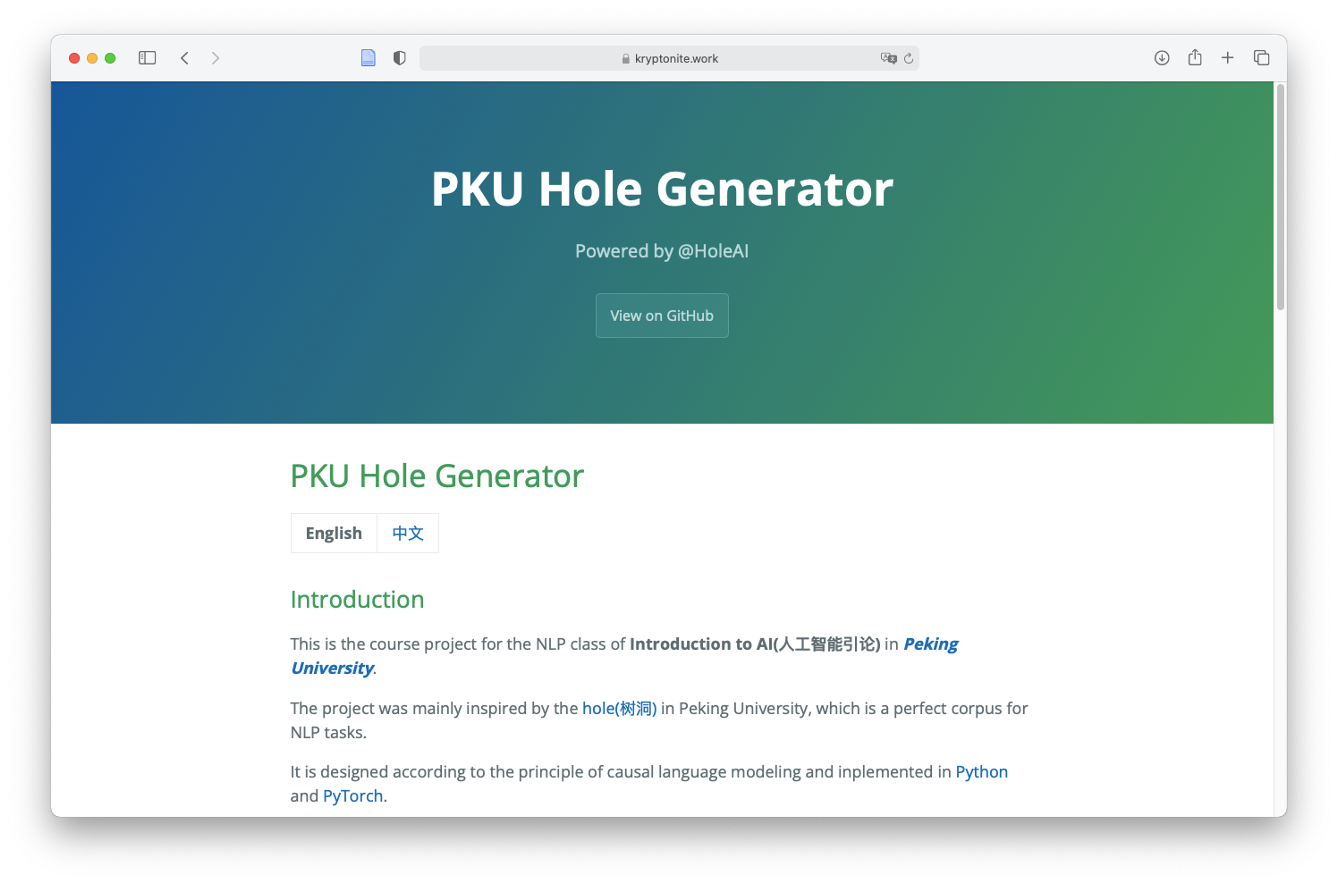
\includegraphics[width=0.9\textwidth]{界面1.png}
        \caption{网站界面}
\end{figure}

在本网站的Let's Try!栏目下,是P大树洞网页版的图标,用户直接点击或点击\href{https://share.streamlit.io/hirojifukuyama/pkuhole/app.py}{此处}即可进入人机交互界面进行游玩。用户可以自行调整模型大小、情绪、长度,进行树洞生成。

人机交互界面如图12所示。

\begin{figure}[!h]
        \centering
        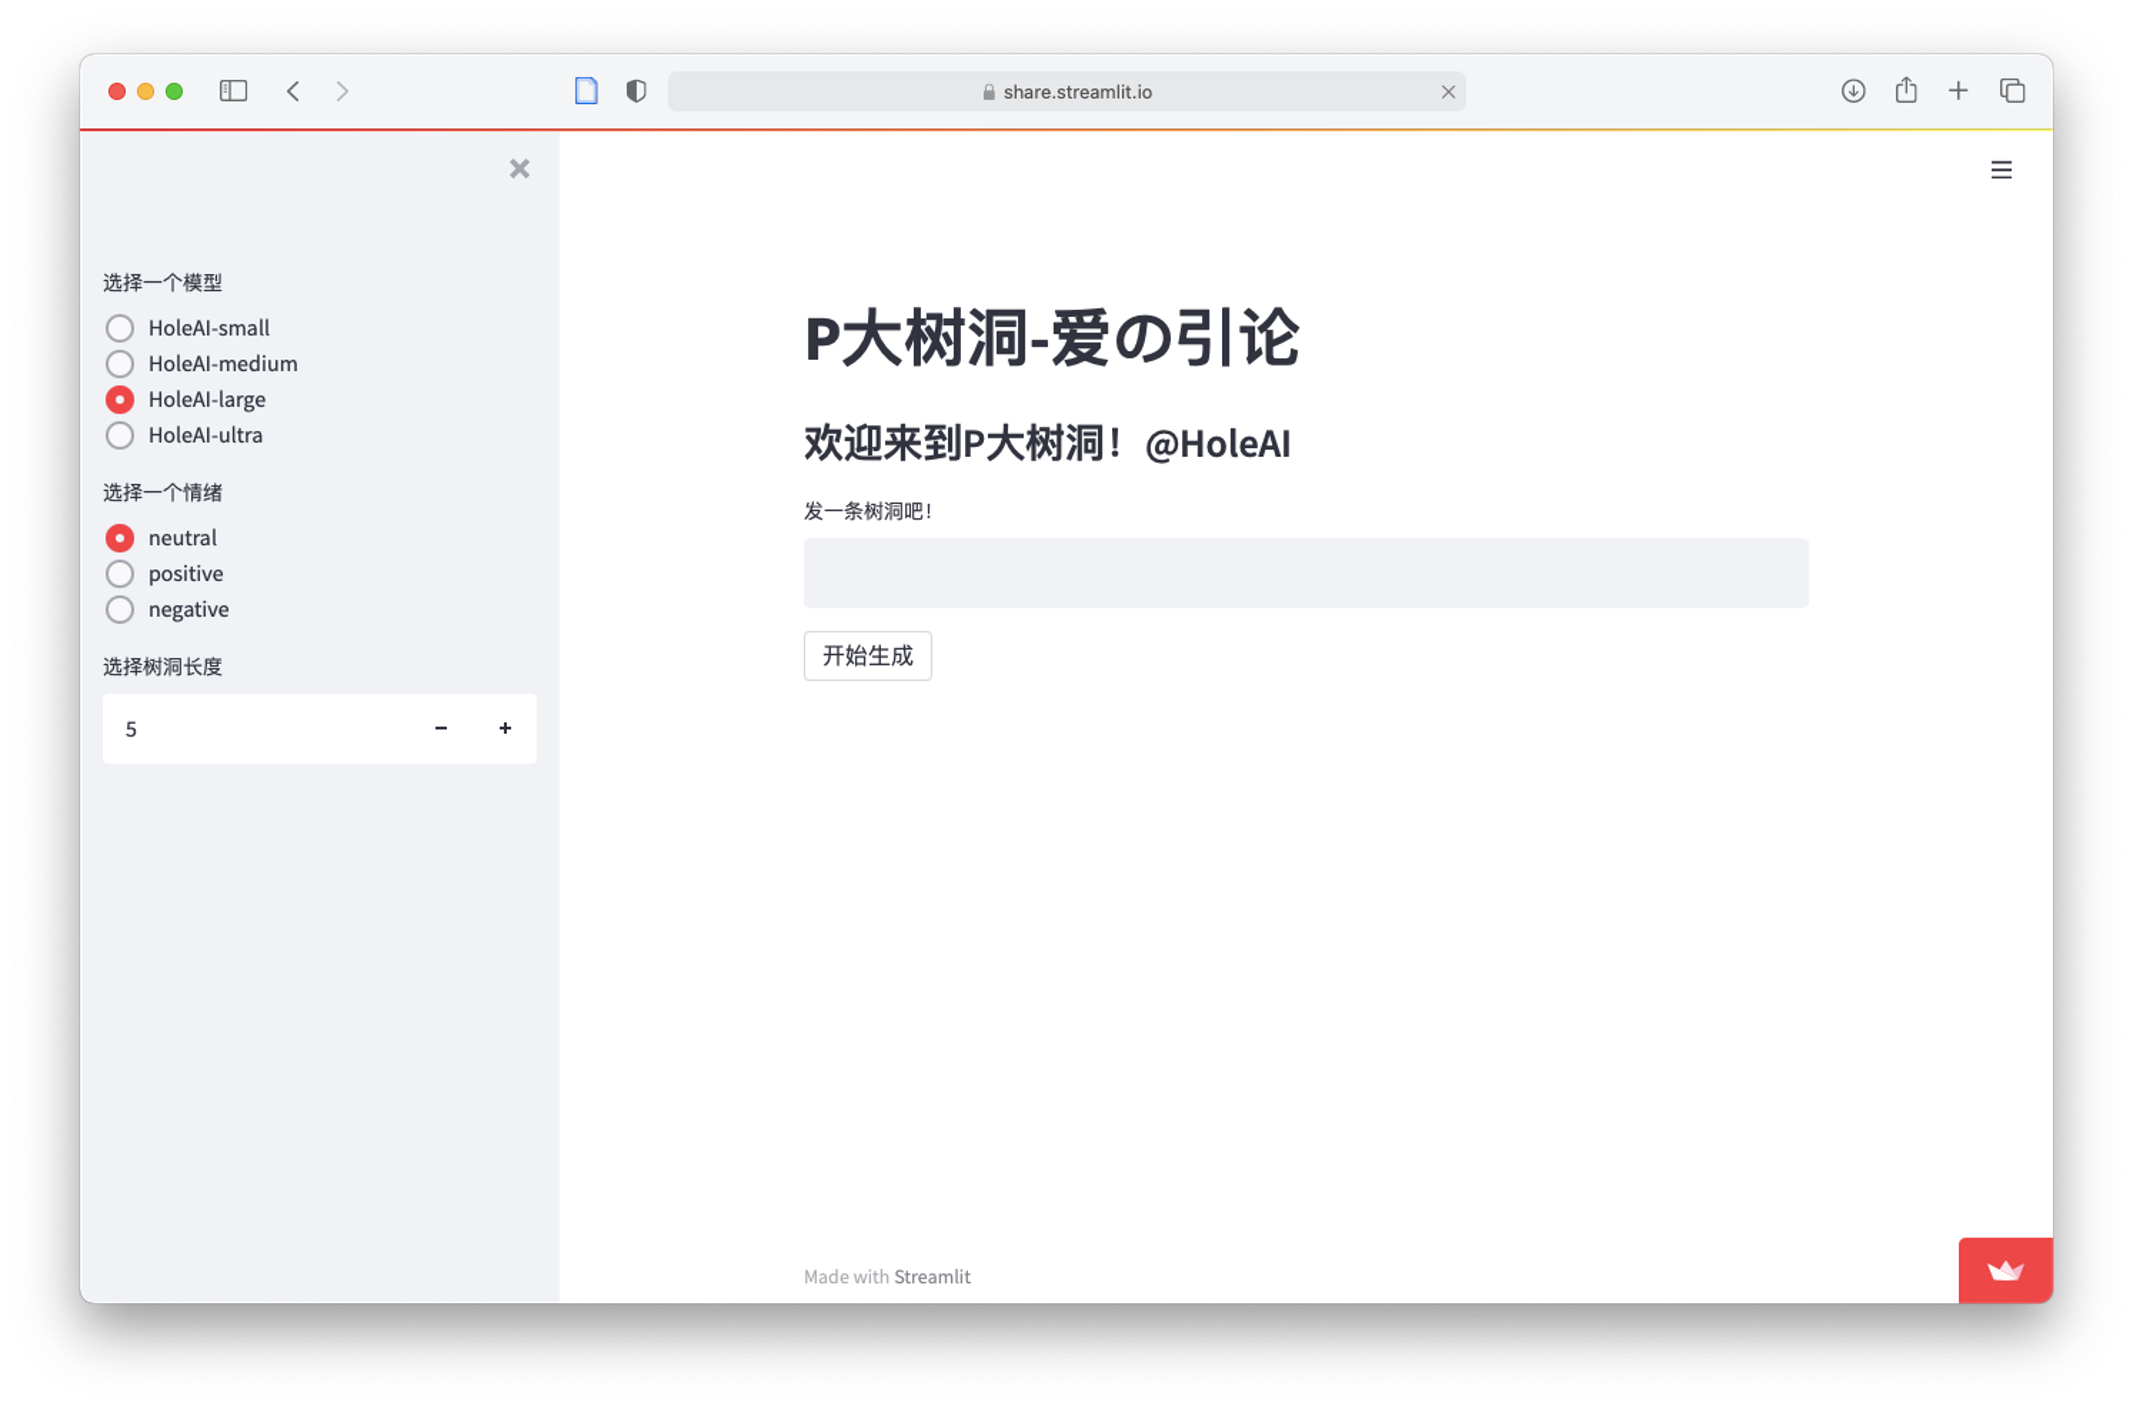
\includegraphics[width=0.9\textwidth]{界面3.png}
        \caption{人机交互界面}
\end{figure}

\section{项目总结}
\subsection{意义}
这个任务十分新颖有趣,而且具有一定社会科学方面的研究价值。

通过本项目,我们刻画了一幅北大学子的群像,我们可以通过模型体验千千万万个“我”的日常生活。
\subsection{挑战}
数据集的缺乏(根本没有)和数据集噪声过多,给我们带来了很大的挑战。我们需要花费大量时间进行数据收集与清洗。

模型大小与数据集大小的匹配则是另一个挑战。我们需要在欠拟合(underfitting)和过拟合(overfitting)之间寻找一种平衡。
\subsection{局限性}
虽然我们的项目制作较为完备,模型效果较好,但依然存在一定局限性:

(1). 数据集较小:由于时间和任务所限,我们无法收集常规情况下巨量的数据,这导致模型出现了不同程度的过拟合现象,如果可以,后续我们也会对数据集的大小和数据分布做出调整。

(2). 模型较为简单:我们采用的模型是经典的LSTM因果语言模型,实现难度较低,并没有fancy的多头注意力机制等等。但是在本项目较小的数据集下,LSTM也可以达到较好的效果,故本问题其实也不构成问题。在对数据集大小进行调整之后,我们也可能会尝试更新的技术,甚至采用预训练模块等等。

\subsection{收获}
通过本项目,我们加深了对Word2Vec、循环神经网络、LSTM的认识,通过实操深入剖析了机器学习的全过程:数据处理、模型搭建、训练评估、模型调参、部署实装,更进一步拓宽了我们对于前沿任务的了解,打开了新世界的大门。

此外,在本项目的完成过程中,我们也在不断学习新的技术,如训练过程可视化、模型部署、网页搭建等等。在这一过程中,看API文档成为了家常便饭,我们也学习了更多人工智能以外的知识。


\section*{小组分工}
\addcontentsline{toc}{section}{小组分工}

匡宇轩:组长。负责规划项目、模型训练、模型部署、前端制作。

陈红韵:组员。负责数据收集、数据清洗、海报制作。

王天源:组员。负责数据收集、汇报制作、报告写作。

\section*{致谢}
\addcontentsline{toc}{section}{致谢}

感谢《人工智能引论》大班课老师的知识讲授,NLP小班课邓志鸿教授的知识讲授与指导,NLP小班课助教学长学姐的指导与帮助。

也感谢本课程独特的课程设置,使我们学会了许多包括但不限于人工智能领域的知识与技能,提高了我们对于互联网的利用能力以及对于个人电脑的熟练操作能力。在这一过程中,我们受益良多。


\begin{thebibliography}{99} 
\addcontentsline{toc}{section}{参考文献}
\setmainfont{Times New Roman}
\bibitem{ref1}Efficient Estimation of Word Representations in Vector Space, Tomas Mikolov, Kai Chen, Greg Corrado, Jeffrey Dean, 2013, \href{https://arxiv.org/abs/1301.3781/}{https://arxiv.org/abs/1301.3781/}
\bibitem{ref2}Long short-term memory, S Hochreiter, J Schmidhuber, 1997, \href{https://pubmed.ncbi.nlm.nih.gov/9377276/}{https://pubmed.ncbi.nlm.nih.gov/9377276/}
\bibitem{ref3}Understanding LSTM Networks, colah's blog, 2015, \href{http://colah.github.io/posts/2015-08-Understanding-LSTMs/}{http://colah.github.io/posts/2015-08-Understanding-LSTMs/}
\end{thebibliography}

\section*{附录}
\addcontentsline{toc}{section}{附录}

\noindent 1.本项目的GitHub地址:\href{https://github.com/HirojiFukuyama/pkuhole/}{https://github.com/HirojiFukuyama/pkuhole/}

\noindent 2.本项目的GitHub Pages:\href{https://kryptonite.work/pkuhole/}{https://kryptonite.work/pkuhole/}

\noindent 3.本项目的人机交互网站:\href{https://share.streamlit.io/hirojifukuyama/pkuhole/app.py/}{https://share.streamlit.io/hirojifukuyama/pkuhole/app.py/}

\noindent 4.训练日志、汇报PPT:详见GitHub仓库

\end{document}
